\chapter{Comprehension of non-morphemic and plural /s/}\label{chapter07}

As illustrated in detail in Section \ref{section02_2}, two comprehension studies are part of this book. This chapter presents the first of these studies on the comprehension of subphonemic differences in word-final /s/. It makes use of real words in isolation with non-morphemic and plural word-final /s/ as items. Effects on comprehension were tested using a number-decision task in a mouse-tracking paradigm. Considering extant models and approaches of speech perception and comprehension, \textsc{H comp}, the ``Mismatch Hypothesis", is investigated. That is, if listeners make use of subphonemic durational differences in the comprehension of different types of word-final /s/, then a mismatch of subphonemic detail and intended meaning is predicted to lead to a) slowed down comprehension processes, and b) deviated mouse trajectories. 

\section{Methdology}\label{section07_1}

\subsection{Participants}\label{section07_1_1}

40 native speakers of New Zealand English took part in the experiment. They were the same participants who also participated in the same-different task described in Chapter \ref{chapter06}. As was the case for the perception experiment, one participant did not respond in any trials and was therefore excluded. The experiment took place at the University of Canterbury, Christchurch, New Zealand, from December 2020 to March 2021.

\subsection{Materials}\label{section07_1_2}

For the present experiment, only real words were used. Recall that words were taken from the British National Corpus (\cite{Davies2004}), following a number of criteria. That is, words had to have a word-final /s/ as part of a voiceless stop plus sibilant coda; they had to be either singular or plural nouns with one syllable; and the number of short monophthong, long monophthong, and diphthong nuclei had to be equally distributed across words for both singular and plural nouns. For singular /s/, it was not possible to fully meet the final criterion as there was only one word with a long monophthong nucleus. Another monomorphemic word with a short monophthong was used instead. As such words had already been sampled for the perception experiment in Chapter \ref{chapter06}, that set of words was used here as well. Additionally, six new words for both singular and plural nouns were added to increase the overall amount of data without a repetition of items (see \cite{Winter2021Grice}, on why repetitions are not desirable). Table \ref{tab:7.1} gives an overview of the complete set of words. As it was not possible to find more monomorphemic words with an even distribution of short monophthongs, long monophthongs, and diphthongs as nuclei, further monomorphemic words with a short monophthong nucleus were used instead.

\begin{table}\fontsize{10}{11}
\caption{Words used as items in the number-decision task. The upper half of words is identical to the set of words used in the perception experiment. The lower half of words was added for the present comprehension experiment}
\label{tab:7.1}
\centering
\begin{tabular}{llll}
\lsptoprule
\multicolumn{2}{c}{Non-morphemic /s/} & \multicolumn{2}{c}{Plural suffix /s/}  \\
\midrule
item            & vowel quality       & item            & vowel quality        \\
\midrule
\textit{mix}    & short               & \textit{books}  & short                \\
\textit{box}    & short               & \textit{steps}  & short                \\
\textit{tax}    & short               & \textit{rights} & diphthong            \\
\textit{coax}   & diphthong           & \textit{points} & diphthong            \\
\textit{hoax}   & diphthong           & \textit{groups} & long                 \\
\textit{corpse} & long                & \textit{parts}  & long                 \\
\textit{lynx}   & short               & \textit{costs}  & short                \\
\textit{flux}   & short               & \textit{crusts} & short                \\
\textit{wax}    & short               & \textit{rates}  & diphthong            \\
\textit{fax}    & short               & \textit{notes}  & diphthong            \\
\textit{lapse}  & short               & \textit{sports} & long                 \\
\textit{fox}    & short               & \textit{cheats} & long                \\
\lspbottomrule
\end{tabular}
\end{table}

The set of twenty-four target items was matched with a set of twenty-four filler items. Half of the filler items were high frequency monosyllabic singular words ending in any consonant but /s/. The other half of the filler items were disyllabic plurals ending in /ɪz/. The type of nucleus, i.e. short or long monophthong and diphthong, was distributed equally across both groups of fillers. All fillers used in the present experiment can be found in Table \ref{tab:7.2}.

\begin{table}\fontsize{10}{11}
\caption{Filler items used in the number-decision task}
\label{tab:7.2}
\centering
\begin{tabular}{llll}
\lsptoprule
\multicolumn{2}{c}{High frequency singulars} & \multicolumn{2}{c}{/ɪz/ plurals}  \\
\midrule
item  & vowel quality                        & item    & vowel quality           \\
\midrule
\textit{end}   & short                                & \textit{kisses}  & short                   \\
\textit{fact}  & short                                & \textit{fences}  & short                   \\
\textit{head}  & short                                & \textit{passes}  & short                   \\
\textit{thing} & short                                & \textit{senses}  & short                   \\
\textit{home}  & diphthong                            & \textit{roses}   & diphthong               \\
\textit{point} & diphthong                            & \textit{houses}  & diphthong               \\
\textit{way}   & diphthong                            & \textit{bases}   & diphthong               \\
\textit{side}  & diphthong                            & \textit{spices}  & diphthong               \\
\textit{car}   & long                                 & \textit{classes} & long                    \\
\textit{world} & long                                 & \textit{horses}  & long                    \\
\textit{room}  & long                                 & \textit{nurses}  & long                    \\
\textit{court} & long                                 & \textit{uses}    & long                   \\
\lspbottomrule
\end{tabular}
\end{table}

The recording of the speech materials took place at a soundproof booth of the Department of Linguistics at the University of Tübingen. For the recording procedure, reading lists were created. On these lists, target items were embedded within the sentence ``He said item to me.", while filler items were embedded within the sentence ``He said item again.". The latter sentence was used for filler items as some of them ended in alveolar stops, /d/ and /t/. Thus, the word \textit{to} following the respective filler items would have potentially led to splicing problems later on due to coarticulatory effects, i.e. the omission of one of the two stops, between filler item and the following word. To keep differences due to phrasal context to a minimum, the decision was made to embed all filler items into the second sentence, including those without word-final alveolar stop. Target items were not embedded within the same sentence but within the one mentioned first, as for word-final /s/ a following stop simplifies the segmentation procedure due to the clear cut-off between friction and closure in the acoustic signal. Examples for target and filler items embedded in the pertinent sentences are given in (14) and (15), respectively.

\ex.
\label{ex:14:sentence14}
He said \textit{hoax} to me.

\ex.
\label{ex:15:sentence15}
He said \textit{world} again.

A trained native-speaker of New Zealand English read the entire reading list aloud for practice before recording the list three times. The recordings were sampled at 44.1 kHz, 16 bit. 

For each item the best of the three recordings was chosen by manual inspection. First, all recordings were analysed using Praat following the segmentation conventions laid out in Section \ref{section04_1_4}. Recordings with production errors, e.g. laughter, stutter or vocal fry, or segmentation difficulties, e.g. the absence of a stop release, were dismissed. Second, the remaining segmented items and filler items were spliced from their surrounding contexts, resulting in audio files only containing the words of interest. Third, the duration of the target and filler items was measured using a Praat script (\cite{deJong2008}) and then analysed in R. The result of this analysis is given as the mean durations presented in Table \ref{tab:7.3}. Lastly, the version closest to the mean duration of its nucleus type was chosen for further use in the experiment to keep durational differences between items to a minimum.

\begin{table}\fontsize{10}{11}
\caption{Mean durations of items and filler items across recordings in seconds}
\label{tab:7.3}
\centering
\begin{tabular}{llccc} 
\lsptoprule
Item type                                                       & ~                                                                   & Short vowel                                           & Long vowel                                            & Diphthong                                              \\ 
\midrule
target items                                                    & \begin{tabular}[c]{@{}l@{}}\textit{mean} \\\textit{sd}\end{tabular} & \begin{tabular}[c]{@{}l@{}}0.576 \\0.109\end{tabular} & \begin{tabular}[c]{@{}l@{}}0.613 \\0.102\end{tabular} & \begin{tabular}[c]{@{}l@{}}0.572 \\0.062\end{tabular}  \\ 
\midrule
\begin{tabular}[c]{@{}l@{}}singular \\filler items\end{tabular} & \begin{tabular}[c]{@{}l@{}}\textit{mean} \\\textit{sd}\end{tabular} & \begin{tabular}[c]{@{}l@{}}0.469 \\0.082\end{tabular} & \begin{tabular}[c]{@{}l@{}}0.467 \\0.035\end{tabular} & \begin{tabular}[c]{@{}l@{}}0.523 \\0.071\end{tabular}  \\ 
\midrule
\begin{tabular}[c]{@{}l@{}}plural \\filler items\end{tabular}   & \begin{tabular}[c]{@{}l@{}}\textit{mean} \\\textit{sd}\end{tabular} & \begin{tabular}[c]{@{}l@{}}0.609 \\0.081\end{tabular} & \begin{tabular}[c]{@{}l@{}}0.607 \\0.056\end{tabular} & \begin{tabular}[c]{@{}l@{}}0.613 \\0.069\end{tabular}  \\
\lspbottomrule
\end{tabular}
\end{table}

Next, for each target the chosen recording was edited so that the word-final /s/ was replaced with another word-final /s/. For recordings of the so-called ``matched condition", this new word-final /s/ was taken from another recording of the same word. If the /s/ was a non-morphemic /s/, its duration was manipulated in such a way that is corresponded to the mean non-morphemic /s/ duration found in \citet{Plag2017}. If the /s/ was a plural /s/, its duration was changed to the mean plural /s/ duration found in the same study, accordingly. For recordings of the so-called ``mismatched condition", the new word-final /s/ was taken from a monomorphemic target in case of a plural base and from a plural target in case of a monomorphemic pseudo-base, i.e. the string of segments of a monomorphemic target without the word-final /s/. The duration of the /s/ was then manipulated in such a way that it corresponded to the mean duration found in \citet{Plag2017} for the other type of /s/. That is, a non-morphemic /s/ was changed to the duration of a plural /s/, and a plural /s/ was changed to the duration of a non-morphemic /s/. This procedure resulted in two recordings per target word, one of the matched condition and one of the mismatched condition. For example, for the monomorphemic target word \textit{mix}, there was an audio stimulus with an /s/ duration of 318 ms for the matched condition and an audio stimulus with an /s/ duration of 283 ms for the mismatched condition. For a plural target like \textit{books}, there was an audio stimulus with an /s/ duration of 283 ms for the matched condition and an audio stimulus with an /s/ duration of 318 ms for the mismatched condition. As the (pseudo-)base and the /s/ in both conditions have been spliced together, a one-sided effect of ``sounding manipulated" on the experiment’s results was ruled out.

\subsection{Procedure}\label{section07_1_3}

The number-decision task was conducted in OpenSesame using the mousetrap plugin for mouse-tracking (\cite{Kieslich2017}). Participants were introduced to the task at hand. They were told that in the following experiment they had to decide whether an audio recording was describing ``one" or ``two or more" entities. They were told to mouse-click on the corresponding button in the top right or top left corner of the screen as quickly as possible. Figure \ref{fig:7_1} illustrates what participants saw on screen for each trial. The participants were also told that if they do not decide on either option within a certain amount of time, the next trial started automatically. Each participant started with six practice trials in which recordings of filler items were used (see the \ref{Supplementary Material}).

\begin{figure}
    \centering
    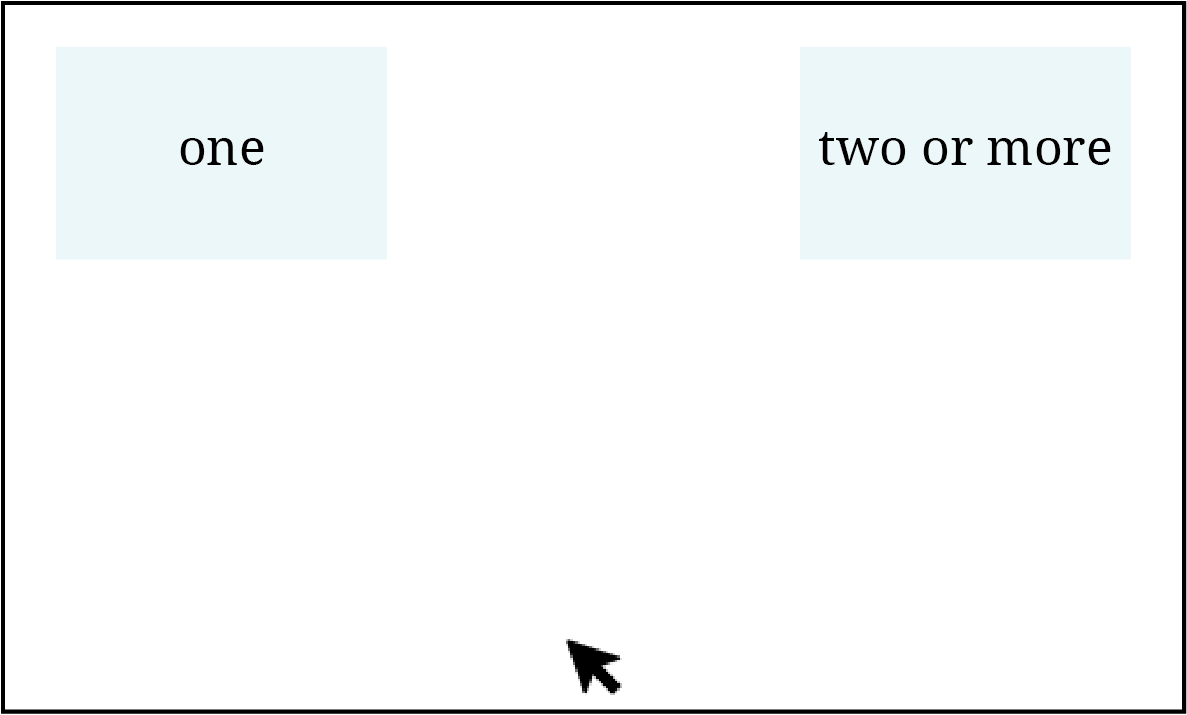
\includegraphics[width=0.7\textwidth]{figures/fig7.1.png}
    \caption{Option display during the comprehension experiment. The mouse cursor indicates the position the mouse was reset to in each trial}
    \label{fig:7_1}
\end{figure}

Each trial was preceded by a stretch of silence of 450 ms. Then, one of the recordings was played, with reaction time and mouse-tracking measurement starting at the onset of the recording. Participants were given a window of 2000 ms starting after the onset of the recording to react, after that a time-out was recorded. The next trial started automatically 2500 ms after the onset of the recording if no reaction was recorded. Mouse-tracks were recorded with a frequency of 100 Hz.

\section{Analysis}\label{section07_2}

The data of the mouse-tracking experiment was analysed in terms of reaction times and mouse trajectories. In the following section, covariates used in the analyses are introduced. Section \ref{section07_2_2} then presents the analysis of reaction time data. The analysis of the mouse-tracks is given in Section \ref{section07_2_3}.

\subsection{Covariates}\label{section07_2_1}

The set of covariates used in the analyses of the present study is similar to that of other studies on phonetic effects of morphological structure (\cite{Pluymaekers2005a, Pluymaekers2005b, Hanique2013Ernestus, Plag2017}; as well as those used in previous chapters of this book). Additionally, some further covariates, which may either influence perception or reactions based on perception, have been introduced. In the following, covariates based on previous studies on morphological structure are described first. For covariates which have been introduced in detail in Chapters \ref{chapter04} and \ref{chapter06}, definitions are briefly repeated for convenience and adapted where necessary. Then, newly introduced covariates are given. Finally, covariates used as random effects are listed.

\textsc{biphoneProbSum}. A covariate based on the summed biphone probability was used as a measure of contextual predictability.

\textsc{monoMultilingual}. To account for potential influences of other L1s besides English, the binary covariate \textsc{monoMultilingual} was introduced. 

\textsc{age}. Subjects’ \textsc{age} was included as it may show an influence on reaction times, with older subjects generally reacting slower than younger subjects (e.g. \cite{Fozard1994}).

\textsc{neighbourhoodDensity}. Neighbourhood densities were included as covariate as the number of neighbours may influence phonetic reduction (e.g. \cite{Gahl2012}). The measure was created using the CLEARPOND database (\cite{Marian2012}). \textsc{neighbourhoodDensity} describes the number of words differing in one segment from the item in question (\cite[3]{Marian2012}).

\textsc{trialNumer}. To account for possible effects of training and fatigue, the number of the trial during the experiment for each of the items per subject was included. 

\textsc{googleFreqLog}. To account for potential effects of frequency (e.g. \cite{Baayen2006, Keuleers2010, Brysbaert2011}), Google frequency was included as covariate as it has been shown that Google frequencies are a robust predictor of reaction times (e.g. \cite{Hendrix2020}). The value of \textsc{googleFreqLog} is the log-transformed number of Google search hits for each individual item as obtained on July 16, 2021.

\textsc{typeOfS}. This binary variable codes whether the pertinent pseudoword is a singular or plural form. It takes the value \texttt{nm} for pseudowords with a non-morphemic word-final /s/ and \texttt{pl} for pseudowords with a plural word-final /s/.

\textsc{musicalInstrument}. It has been shown that advanced players of musical instruments show an increased performance of phonological perception and of detecting durational differences in speech (\cite{Anvari2002, Milovanov2009}). Thus, information on how regularly each subject plays a musical instrument was added as covariate.

\textsc{condition}. The \textsc{condition} variable is the explanatory variable of interest. Its levels are matched and mismatched and refer to the ``matched" and ``mismatched" conditions introduced by the creation of the audio stimuli used in the present experiment. Recall from Section \ref{section07_1_2} that in matched stimuli (pseudo-)base and duration of the word-final /s/ match up, while there is a discrepancy of (pseudo-)base and word-final /s/ duration for mismatched stimuli. 

\textsc{correct}. \textsc{correct} is a binary variable coding whether the answer clicked on by the subject in the relevant trial is the correct answer in regard to the (pseudo-)base of the stimulus.

\textsc{dominantHand}. Reaction times between the dominant and the non-domi-nant hand may differ (\cite{Gignac2004}). The information which hand was dominant in each subject was added as a covariate, as all participants used the same hand (i.e. their right hand) to use the mouse.

\textsc{order}. This variable codes the order of X and Y coordinates, i.e. their chronological order in the observed mouse-tracks. \textsc{order} was incorporated as a variable to account for the natural sequence of coordinates, i.e. to account for potential influences of auto-correlation. 

\textsc{videoGames}. It has been shown that playing video games can reduce reaction times (e.g. \cite{Dye2009}). The relative frequency of how often a subject engages in playing video games was therefore included as a categorical covariate called \textsc{videoGames}.

\textsc{item}. For each item, its orthographic representation was contained as level of item. This covariate was used as a random effect to account for potential differences between individual targets not covered by other covariates.

\textsc{subject}. \textsc{subject} ID was included to account for inter-speaker differences in perception.

Closer inspection of the covariates describing subject characteristics, i.e. \textsc{dominantHand}, \textsc{monoMultilingual}, \textsc{musicalInstrument}, and \textsc{videoGames}, revealed that for all of these variables there was an uneven distribution of subjects across levels. That is, only 7 \% (n = 117) of trials had \texttt{left} for \textsc{dominantHand}, and only 19 \% (n = 302) of trials had \texttt{multilingual} for \textsc{monoMultilingual}. For \textsc{musicalInstrument} and \textsc{videoGames}, which both have five levels, the distribution is even more uneven. The level least represented in \textsc{musicalInstrument} is \texttt{very often} with 6 \% (n = 95), while the most represented level is \texttt{never} with 41 \% (n = 666). A similar picture is found for \textsc{videoGames}, where the least represented level is \texttt{often} with 8 \% (n = 126), while the level most represented is \texttt{never} with 38 \% (n = 621). The uneven distribution of data points across variables and their levels also led to some ``empty cells" within the possible combinations of levels across covariates. For example, all subjects for which the value of \textsc{monoMultilingual} is \texttt{multilingual} have \texttt{right} as their \textsc{dominantHand}. There are no \texttt{multilingual} subjects who play a musical instrument \texttt{often} or \texttt{very often} and no \texttt{multilingual} subjects who \texttt{often} play \textsc{videoGames}. Further, all \texttt{left}-handed subjects \texttt{never} play a \textsc{musicalInstrument} and they \texttt{rarely} or \texttt{never} play \textsc{videoGames}. Due to this issue of sparse data and as for such variables with levels underrepresented in the sample it is unclear whether effects, found or not found, are due to a real effect of the variable or simply an artefact of chance. It was thus decided to drop the following covariates: \textsc{dominantHand}, \textsc{musicalInstrument}, and \textsc{videoGames}. \textsc{monoMultilingual} is retained for the analyses as the variable is directly related to language and because the variable has been used in other analyses of this book.

\subsection{Reaction times}\label{section07_2_2}

The present reaction time data were analysed using piece-wise additive mixed models (PAMMs; \cite{Bender2018etal}, and as briefly introduced in Section \ref{section03_2_2}). In the following, I will introduce the basics of PAMMs; the interested reader is referred to \citet{Hendrix2020} for a more thorough introduction using linguistic data and to \citet{Bender2018etal} for a more detailed mathematical implementation. 

PAMMs are a relatively novel technique of time-to-event analysis, that is they model the time until an event of interest occurs. The event of interest in the present number-decision task is the ``one" or ``two or more" response to a stimulus. Thus, the dependent variable in a PAMM is the instantaneous probability of a response as it evolves over time, not the reaction time itself (\cite{Hendrix2020}). Using PAMMs allows for an insight into the temporal dynamics of predictor effects. Hence, PAMMs do not only capture effects covering entire trials but also effects that occur only during particular parts of trials or show different effects during different parts of trials. A central function of time-to-event analysis is the probability density function $F(t$):

\begin{equation}
\label{eq:Ft}
    F(t)=\int_{-\infty}^{t}f(x)dx=P(T\leq t).
\end{equation}

The probability density function describes the probability that the response time $T$ is smaller than or equal to a given time $t$. Closely related to the probability density function is the survival function:

\begin{equation}
\label{eq:St}
    S(t)=1-F(t)=P(T>t).
\end{equation}

The survival function describes the probability of the time at which the event of interest occurs $T$ being greater than at a given time $t$. For the present experiment, the survival function describes the probability that subjects did not yet respond to a stimulus at time $t$. However, the mathematical properties of the function are not optimal for modelling purposes (\cite{Hendrix2020}). Thus, PAMMs make use of a closely related function, the hazard function. The hazard function describes the instantaneous probability that the event of interest occurs at time $t$, given that the event did not occur already. It is defined as

\begin{equation}
\label{eq:lambdat}
\lambda(t)=\lim \limits_{dt \to \infty}\frac{P(t\leq T\leq t\, |\, T\geq t)}{dt}=-\frac{d}{dt}log(S(t)).
\end{equation}

Before one can create PAMMs on reaction time data, though, the data has to be transformed. That is, the modelling of PAMMs requires data in the so-called piece-wise exponential data format (\cite{Bender2018a}). While standard linear models (e.g. LMERs) or non-linear regression models (e.g. GAMMs) would use reaction times as dependent variable, PAMMs use the information on whether or not a stimulus was responded to at time $t$ as dependent variable. The piece-wise exponential data format splits the time each stimulus is at risk of being responded to into $J$ intervals. The intervals $(k_{j-1},k_j ],j=1…J$ are defined by the cut points $K_0<⋯<K_J$. The choice of cut points is arbitrary (\cite{Hendrix2020}); over-fitting is prevented through penalization of wiggliness (e.g. \cite{Wood2017}). $t_j$ then equals $k_j$, i.e. $t$ is derived from the defined cut points $K$. Following \citet{Hendrix2020}, cut points at the extreme ends of the response time distribution were opted for. That is, cut points prior 770 ms, as only 11 trials (0.68 \%) were responded to earlier than 770 ms after stimulus onset, and after 1970 ms, as only 12 trials (0.74 \%) were responded to later than 1970 ms after stimulus onset, were excluded. An example of the transformed data is given in Table \ref{tab:7.4}.

\begin{table}\fontsize{10}{11}
\caption{Example of the piece-wise exponential data format for one stimulus instantiating the word \textit{box}}
\label{tab:7.4}
\centering
\begin{tabular}{lllrrrrr} 
\lsptoprule
row & \textsc{ID}  & \textsc{item} & \textsc{tstart}  & \textsc{tend}    & \textsc{interval}          & \textsc{offset} & \textsc{status}  \\ 
\midrule
1   & 256 & box  & 0.00    & 817.00  & (0.00,817]        & 6.706  & 0       \\
2   & 256 & box  & 817.00  & 922.00  & (817.00,922.00]   & 4.654  & 0       \\
3   & 256 & box  & 922.00  & 977.00  & (922.00,977.00]   & 4.007  & 0       \\
…   & …   & …    & …       & …       & …                 & …      & …       \\
26  & 256 & box  & 1345.92 & 1363.00 & (1345.92,1363.00] & 2.838  & 0       \\
27  & 256 & box  & 1363.00 & 1379.08 & (1363.00,1379.08] & 2.079  & 1       \\
\lspbottomrule
\end{tabular}
\end{table}

The piece-wise exponential data format contains a separate row for each interval for each stimulus. In each row, the start (\textsc{tstart}) and end point (\textsc{tend}) of the interval are given. The end points are included as predictor in a PAMM to estimate the hazard function over time. The \textsc{offset} variable provides information about the exact response time for each stimulus. For intervals in which no response was recorded (rows 1 to 26), the \textsc{offset} is the log-transformed duration of the interval, while for intervals in which a response was recorded (row 27), the \textsc{offset} is the log-transformed value of the difference of the exact time of response and the start of the interval, i.e. \textsc{tstart}. Please note the notation of the interval information: $(k_{j-1},k_j]$ indicates that the first value, $k_{j-1}$, is included in the interval while the second value, $k_j$, is not. $k_j$, then, is the starting value of the following interval. The dependent variable in PAMMs, \textsc{status}, is a binary variable, which encodes whether a word was responded to (\texttt{1}) or not (\texttt{0}) in the pertinent interval. 

A PAMM is then defined as follows:

\begin{equation}
\label{eq:lambdatxi}
\lambda(t|x_{i})=\lambda_{0}(t_{j})exp\left ( \sum_{k=1}^{p}f_{k}(x_{i,k},t_{j})+b_{\ell_{i}} \right ),\: \forall\, t \in (K_{j-1},K_{j}]
\end{equation}

with the predictor values $x_i$ for stimulus $i$ defining the hazard function $\lambda(t|x_{i})$ at all time points $t$ in the interval $j≔(K_{j-1},K_j]$. $λ_0 (t_j)$ is the baseline hazard for time interval $j$, $f_k (x_{i,k},t_j)$ are smooth functions for predictor $k∈1,…,p$ for each time point $t$ in the interval $j$, and $b_{\ell_{i}}$ are random intercepts associated with group $l∈1,…,L$ to which stimulus $i$ belongs (\cite{Hendrix2020}).

\subsubsection{Overview of the data}\label{section07_2_2_1}

An overview of all variables used in the PAMM modelling process and their distribution is given in Table \ref{tab:7.5} and Table \ref{tab:7.6}.

\begin{table}\fontsize{10}{11}
\caption{Summary of the dependent variable and the numerical predictors in the final data set}
\label{tab:7.5}
\centering
\begin{tabular}{lrrrr} 
\lsptoprule
Dependent variable   & \multicolumn{4}{l}{Levels}                                      \\ 
\midrule
\textsc{status}               & \multicolumn{2}{l}{0:
  41471} & \multicolumn{2}{l}{1:
  1616}  \\ 
\midrule
Numerical predictors & Mean     & St. Dev.            & Min     & Max                  \\ 
\midrule
\textsc{biphoneProbSum}       & 0.015    & 0.009               & 0.002   & 0.043                \\
\textsc{age}                  & 23.313   & 5.575               & 18.000  & 39.000               \\
\textsc{neighbourhoodDensity} & 17.068   & 10.039              & 1.000   & 34.000               \\
\textsc{trialNumber}          & 36.358   & 20.678              & 1.000   & 72.000               \\
\textsc{googleFreqLog}        & 9.190    & 0.787               & 7.658   & 10.302               \\
\textsc{tend}                 & 1234.455 & 212.414             & 817.000 & 1960.000             \\
\lspbottomrule
\end{tabular}
\end{table}





\begin{table}\fontsize{10}{11}
\caption{Summary of the dependent variables and the explanatory variable in the final data set}
\label{tab:7.6}
\centering
\begin{tabular}{lllll} 
\lsptoprule
Categorical predictors & Levels & ~                               & ~ & ~                                     \\ 
\midrule
\textsc{typeOfS}                & \multicolumn{2}{l}{\texttt{nm}: 22159}            & \multicolumn{2}{l}{\texttt{pl}:
  20928}           \\
\textsc{correct}                & \multicolumn{2}{l}{\texttt{no}: 7795}             & \multicolumn{2}{l}{\texttt{yes}: 35292}            \\
\textsc{monoMultilingual}       & \multicolumn{2}{l}{\texttt{monolingual}:
  37578} & \multicolumn{2}{l}{\texttt{multilingual}:
  5509}  \\
\textsc{item}                   & 24     & ~                               & ~ & ~                                     \\
\textsc{subject}                & 39     & ~                               & ~ & ~                                     \\ 
\midrule
Explanatory variable   & Levels & ~                               & ~ & ~                                     \\ 
\midrule
\textsc{condition}              & \multicolumn{2}{l}{\texttt{matched}:
  21176}     & \multicolumn{2}{l}{\texttt{mismatched}:
  21911}   \\
\lspbottomrule
\end{tabular}
\end{table}

\subsubsection{Fitted models}\label{section07_2_2_2}

A PAMM was fitted with STATUS as dependent variable and \textsc{biphoneProbSumBin}, \textsc{age}, \textsc{neighbourhoodDensity}, \textsc{trialNumer}, and \textsc{googleFreqLog} as smooth terms. For each smooth, time-varying predictor effects were allowed for by including tensor product interactions between time, i.e. \textsc{tend}, and the predictor itself (see \cite{Wood2017}, for further details on tensor product interactions). To ensure interpretable results, the predictor smooths were limited to four basis functions, and time-by predictor interactions were limited to fourth order non-linearities. No limits were set on the smooth for time. The categorical covariates \textsc{typeOfS}, \textsc{condition}, \textsc{correct}, and \textsc{monoMultilingual} were included as parametric effects. The covariates \textsc{item} and \textsc{subject} were included as random smooth terms. Starting from this initial model, the modelling process proceeded as introduced in Section \ref{section03_2_2}. It was found that the \textit{k}-index value of the tensor product interaction of \textsc{tend} and \textsc{trialNumber} was $0.006$. Recall that \textit{k}-values well below $0.05$ indicate potentially missed patterns in the residuals. Re-modelling with a limit of a sixth instead of a fourth order non-linearity resolved the issue. The prediction error curve (e.g. \cite{Mogensen2012}) displaying the Brier score (e.g. \cite{Brier1950, Gerds2006, Bradley2008}) of the final model is displayed in Figure \ref{fig:7_2}. As a reference, the Brier score of the Kaplan-Meier estimate (\cite{Kaplan1958}) is given. The Brier score measures the accuracy of probabilistic predictions. The lower its value for a set of predictions, the better the predictions are calibrated. The range of possible Brier score values is $(0,1)$. In the present case, the Brier score of the PAMM is considerably better than the Brier score of the Kaplan-Meier estimate. This indicates that the inclusion of the covariates in the PAMM improves the accuracy of the model predictions. 

\begin{figure}
    \centering
    \includesvg[]{figures/fig7.2.svg}
    \caption{Comparison of the Brier scores of the fitted PAMM and its Kaplan-Meier estimate equivalent}
    \label{fig:7_2}
\end{figure}

A valid question to ask when using novel statistical methods is whether the extra work is worth the trouble, i.e. whether the novel methods result in, for example, models with a higher fit. To answer this question for the present case, an LMER model with reaction time as dependent variable was fitted. As fixed effects the parametric effects and smooth terms given in the PAMM formula (i.e. \textsc{biphoneProbSum, age, neighbourhoodDensity, trialNumber, googleFreqLog, typeOfS, condition, correct} and \textsc{monoMultilingual}) were specified. \textsc{item} and \textsc{subject} were included as random intercepts. The modelling process then followed the procedure introduced in Section \ref{section03_2_1}. The final LMER model and the PAMM model were then compared by their AIC values: The AIC value of the LMER model was $21,811.36$, the AIC value of the PAMM was $15,360.92$. That is, the AIC value of the PAMM was smaller by $6,450.438$ points. Thus, the PAMM shows a significant better fit. Regarding its model formula, the final LMER model only contained \textsc{trialNumber} and \textsc{monoMultilingual} as fixed effects and \textsc{subject} as random effect. To briefly foreshadow the results presented in the next section, the LMER model did not find a significant effect for \textsc{age}, while the PAMM did find a significant interaction of \textsc{age} and time (\textsc{tend}). This difference then denotes the potentially most prominent advantage of PAMMs: As mentioned in Section \ref{section07_2_2}, PAMMs allow for an insight into the temporal dynamics of predictor effects, while LMER models fitted to the raw reaction time data do not. Overall, fitting PAMMs instead of LMER models appears to be worthwhile for the present data.

\subsubsection{Results}\label{section07_2_2_3}

Main effects of the following predictors were found: \textsc{tend}, \textsc{trialNumber}, and \textsc{monoMultilingual}. Additionally, the interactions between \textsc{tend} and \textsc{trial} and between \textsc{tend} and \textsc{age} reached significance. The results of the PAMM fitted to the reaction time data is given in Table \ref{tab:7.7}. For the parametric terms, I provide the β estimates and the corresponding standard errors (SE), \textit{z}-values, and \textit{p}-values. For the smooth terms, the estimated degrees of freedom, the reference degrees of freedom, the χ\textsuperscript{2} values, and the \textit{p}-values are given. The R script used for the analyses as well as the data set can be found in the \ref{Supplementary Material}.

\begin{table}\fontsize{10}{11}
\caption{Summary of the PAMM fitted to status with \textsc{typeOfS}, \textsc{condition}, \textsc{correct}, and \textsc{monoMultilingual} as parametric effects, \textsc{biphoneProbSum}, \textsc{age}, \textsc{NeighbourhoodDensity}, \textsc{trialNumber}, and \textsc{GoogleFreqLog} as smooth terms, and \textsc{item} and \textsc{subject} as random smooth terms}
\label{tab:7.7}
\centering
\begin{tabular}{lrrrr} 
\lsptoprule
Parametric Terms             & Estimate & SE     & z value  & \textit{p}-value  \\ 
\midrule
(Intercept)                  & -6.867   & 0.152  & -45.238  & 0.000             \\
\textsc{typeOfS}\texttt{pl}                    & 0.133    & 0.101  & 1.321    & 0.187             \\
\textsc{monoMultilingual}\texttt{multilingual} & 0.788    & 0.302  & 2.614    & 0.009             \\
\textsc{condition}\texttt{mismatched}          & -0.044   & 0.051  & -0.858   & 0.391             \\
\textsc{correct}\texttt{yes}                   & 0.061    & 0.075  & 0.810    & 0.418             \\ 
\midrule
Smooth Terms                 & edf      & Ref.df & Chi.sq   & \textit{p}-value  \\ 
\midrule
\textsc{tend}                         & 7.830    & 8.653  & 1516.374 & 0.000             \\
\textsc{GoogleFreqLog}                & 1.002    & 1.003  & 0.468    & 0.682             \\
\textsc{biphoneProbSum}               & 1.001    & 1.002  & 0.989    & 0.321             \\
\textsc{NeighbourhoodDensity}         & 1.300    & 1.495  & 1.760    & 0.391             \\
\textsc{age}                          & 1.002    & 1.002  & 3.258    & 0.071             \\
\textsc{trialNumber}                  & 1.001    & 1.002  & 64.063   & 0.000             \\ 
\midrule
Interactions                 & edf      & Ref.df & Chi.sq   & \textit{p}-value  \\ 
\midrule
\textsc{tend,
  GoogleFreqLog}        & 1.352    & 1.613  & 0.580    & 0.753             \\
\textsc{tend,
  biphoneProbSum}       & 1.539    & 1.882  & 1.238    & 0.423             \\
\textsc{tend,
  NeighbourhoodDensity} & 1.016    & 1.031  & 1.215    & 0.281             \\
\textsc{tend,
  age}                  & 5.942    & 7.321  & 20.257   & 0.007             \\
\textsc{tend,
  trialNumber}          & 2.982    & 3.012  & 50.727   & 0.000             \\ 
\midrule
Random Smooth Terms          & edf      & Ref.df & Chi.sq   & \textit{p}-value  \\ 
\midrule
\textsc{item}                         & 3.112    & 20.000 & 3.879    & 0.267             \\
\textsc{subject}                      & 34.184   & 36.000 & 505.162  & 0.000             \\
\lspbottomrule
\end{tabular}
\end{table}

Figure \ref{fig:7_3} shows the distribution of raw reaction times for items in the matched and mismatched \textsc{condition}. On average, matched stimuli are reacted to after 1374 ms, while mismatched stimuli are reacted to after 1388 ms. 

\begin{figure}
    \centering
    \includesvg[]{figures/fig7.3.svg}
    \caption{Observed reaction times for trials of matched and mismatched items. The dot represents the median, the horizontal line indicates the mean. The violin shapes represent rotated density plots describing the distribution of the data}
    \label{fig:7_3}
\end{figure}

Taking into account this rather small difference of 14 ms and the overall similarity of shape between the two RT distributions, it is not surprising that \textsc{condition} as a predictor did not reach significance in the PAMM. The significant effects found instead are explained in the following.

Panel A of Figure \ref{fig:7_4} shows the partial effect ($p<0.001$) of the categorical variable \textsc{monoMultilingual}. It is found that \texttt{multilingual} subjects show a higher probability of earlier responses than \texttt{monolingual} subjects. This effect is visible in the distribution of the raw RT data (Panel B) as well. However, one should take this effect with caution as the number of \texttt{multilingual} subjects’ data points (n = 302) is much smaller than the number of \texttt{monolingual} subjects’ data points (n = 1326). 

\begin{figure}
    \centering
    \includesvg[]{figures/fig7.4.svg}
    \caption{Partial main effect of \textsc{monoMultilingual} (A), and observed reaction times for monolingual and multilingual subjects (B)}
    \label{fig:7_4}
\end{figure}

A significant main effect of \textsc{trialNumber} ($χ^{2}=63.890, p<0.001$) was found, as well as a significant interaction between time and \textsc{trialNumber} ($χ^{2}=50.205,$ $p<0.001$). The effect of \textsc{trialNumber} is modulated by the interaction with time as shown in Figure \ref{fig:7_5}. Warmer colours indicate higher hazard rates.\footnote{Note that readers of a black and white version of this book should rely on the numbers on the lines instead. Warmer colours correspond to positive values, while cooler colours correspond to negative values.} That is, the interaction between \textsc{trialNumber} and time indicates that the increase of the instantaneous probability of a response for later trials is especially prominent during the early stages of the response window. Later on, the facilitatory main effect of \textsc{trialNumber} is offset by an opposite effect of the partial interaction between \textsc{trialNumber} and time.

\begin{figure}
    \centering
    \includesvg[]{figures/fig7.5.svg}
    \caption{The effect of the interaction between \textsc{trialNumber} and time. Warmer colours indicate higher hazard rates}
    \label{fig:7_5}
\end{figure}

Finally, a significant interaction between time and \textsc{age} ($χ^{2}=20.151, p<0.05$) was found. This effect is illustrated in Figure \ref{fig:7_6}. Again, warmer colours indicate higher hazard rates. That is, the interaction between \textsc{age} and time indicates that the increase of the instantaneous probability of a response for ages between approximately 23 and 28 years is especially prominent during the mid to late stages of the response window, i.e. around 1400 ms to 1750 ms into the trial. The grey area indicates ranges for which no or not enough data was available to the model.\footnote{For readers of a black and white version of this book this area should be visible as dark grey area, which is almost shaped like a perfect rectangle.} As only few subjects (n = 4) contribute to the data above the grey area, shown effects should be interpreted with caution. 

\begin{figure}
    \centering
    \includesvg[]{figures/fig7.6.svg}
    \caption{The effect of the interaction between \textsc{age} and time. Warmer colours indicate higher hazard rates}
    \label{fig:7_6}
\end{figure}

\subsubsection{Interim summary: Reaction times}\label{section07_2_2_4}

Overall, \textsc{condition} as a predictor did not reach significance in the PAMM. That is, participants responded with the same speed to matched and mismatched items. Instead, effects of \textsc{monoMultilingual}, \textsc{trialNumber}, and \textsc{age} were found.

\subsection{Mouse-tracks}\label{section07_2_3}

Mouse-tracking data elicited in OpenSesame using the \texttt{mousetrap} plugin (\cite{Kieslich2017}) was worked with in R using the \texttt{mousetrap} package (\cite{Kieslich2019}). Following standard procedures, the raw mouse-tracking data was first transformed to the so-called ``mousetrap data format" using the \texttt{mt\_import\_mousetrap} function. This function transforms the vectors of X and Y coordinates and their associated timestamps into meaningful row-by-row data for further processing. Then, trials without mouse-movement were discarded. During the experiment subjects clicked on the right and left options on screen (see Section \ref{section07_1_3}). To make mouse-tracks to both sides comparable, those towards the right option were mirrored vertically. Finally, all mouse-tracking data was time-normalised. Time-normalisation is commonly performed if the number of recorded X and Y coordinates varies across trajectories, which typically is the case for trajectories of differing reaction times. After time-normalisation with a constant number of equally sized time steps, all trajectories have the same number of recorded positions, and the positions at different relative time points can be compared across trajectories. 

Figure \ref{fig:7_7} shows the mean trajectory of all spatially adjusted and time-norma-lised mouse-tracks used in the present analysis in the lower left panel. The panel on top displays the overall distribution of all X coordinates, with a clear peak around a value of $0$. The panel on the right shows the overall distribution of all Y coordinates, with a clear peak around a value of about $380$. The peaks correspond to the position to which the mouse was reset to for each trial.

\begin{figure}
    \centering
    \includesvg[]{figures/fig7.7.svg}
    \caption{Mean trajectory of all spatially adjusted and time-normalised mouse-tracks (lower left), and density distribution of X and Y coordinates (on top and on the right, respectively)}
    \label{fig:7_7}
\end{figure}

As all mouse-tracks were spatially transformed, they all move towards the left option in the very end. Thus, one can also derive some further information from Figure \ref{fig:7_7}. That is, taking into account the right part of the density plot of the X coordinates, it becomes visible that subjects in some trials must have deviated from a direct path. For example, if the final answer was the left option, at some point during the trial the mouse must have been on the (far) right part of the screen.

Figure \ref{fig:7_8} displays the average mouse-tracks for the variable of interest, \textsc{condition}. Judging from the raw aggregated data alone, a difference between mouse-tracks of matched and mismatched trials is visible. In the following, I will explain how the statistical analysis of the mouse-tracking data investigating the difference between matched and mismatched trials was conducted.

\begin{figure}
    \centering
    \includesvg[]{figures/fig7.8.svg}
    \caption{Mean trajectories of mouse-tracks for matched and mismatched item trials}
    \label{fig:7_8}
\end{figure}

Initially, regular Gaussian generalised additive mixed models were fitted to the X and Y coordinates of the mouse-track data. However, model criticism revealed that the fitted GAMMs showed rather problematic amounts of autocorrelation. Autocorrelation, or more specifically temporal spatial autocorrelation, is the association between data values over time. Depending on the sign of autocorrelation, model estimates can either be over- or underestimated (\cite{Charlton2009}). Thus, models with a high degree of autocorrelation are unreliable in their predictions. It was therefore decided to use QGAMs instead of GAMMs. QGAMs, as briefly introduced in Section \ref{section03_2_2}, are additive quantile regression models. They are a distribution-free method for estimating the predicted values for any given quantile of the response distribution. As QGAMs are a relatively new tool within the toolbox of GAMs, I will explain the main characteristics of QGAMs as introduced by \citet{Fasiolo2021} in the following. The interested reader is referred to the aforementioned paper for a more thorough mathematical introduction. 

Quantile regression, as conducted by QGAMs, aims at modelling the $\tau$th quantile of the response, $y$, conditionally on a $p$-dimensional vector of covariates, $x$, with $k$ basis functions, where $\tau \in (0,1)$. The $\tau$th quantile then is 

\begin{equation}
\label{eq:mu}
    \mu=\inf \left \{ y:F(y|x)\geq \tau \right \}.
\end{equation}

This can also be defined as the minimizer of the expected loss

\begin{equation}
\label{eq:Lmux}
    L(\mu|x)=\int \rho_{\tau}(y-\mu)dF(y|x),
\end{equation}

where the quantity $\rho_{\tau}(z)$ is the pinball loss (\cite{Koenker2005, Gneiting2011}), which attributes different weights to observations depending on the sign of the residuals $z$:

\begin{equation}
\label{eq:rhotauz}
    \rho_{\tau}(z)=\left \{ \begin{matrix}
    (\tau+1)z\ & \mathrm{if}\, z<0\\ 
    \tau z & \mathrm{if} \, z\geq 0
    \end{matrix} \right..
\end{equation}

The quantile estimator is thus penalised to prevent overfitting, and the amount of penalisation is determined by the so-called learning rate, which determines the relative weight of the loss and the penalty. A QGAM then is defined as

\begin{equation}
\label{eq:mutaui}
    \mu_{\tau}(i)=\beta_{0}+\sum_{k=1}^{\rho}f_{k}(x_{i,k})+b_{\ell_{i}}.
\end{equation}

The term $\sum_{k=1}^{\rho}f_{k}(x_{i,k})$ can represent either a linear effect or a non-linear effect without a predefined structure. $b_{\ell_{i}}$ models random intercepts for group $\ell=1,...,L$ to which observation $i$ belongs, and $\beta_{0}$ is the y-intercept.

In less technical terms, QGAMs make use of the general features of GAMs in modelling linear and non-linear effects as well as random effects. Instead of taking into account the whole range of data for their fitting process, each QGAM is restricted to a given conditional quantile of the data. Splitting the data into ten equally sized conditional quantiles, one can infer, for example, the following. Let us assume that the data is ordered from lowest to highest value, as is the case for the density plots of Figure \ref{fig:7_9} Then the so-called $0.1$ quantile (Panel A) will consist of the first 10 \% of data, that is the tenth of the data consisting of the lowest values. The $0.5$ quantile (Panel B), then, consists of the first 50 \% of the data, and the $0.9$ quantile (Panel C) contains all data but the highest 10 \%. 

\begin{figure}
    \centering
    \includesvg[]{figures/fig7.9.svg}
    \caption{Illustration of the three conditional quantiles $0.1$ (Panel A), $0.5$ (Panel B), and $0.9$ (Panel C) in blue}
    \label{fig:7_9}
\end{figure}

Fitting QGAMs to several of these quantiles allows for a detailed picture of the effects to be investigated. If an effect is present in the $0.1$ quantile but no longer present in the $0.3$ quantile, for example, one can conclude that the effect is significant for data of the lowest 10 \% but loses its significance when taking into account higher valued data points. If the same effect then regains its significance in the $0.5$ quantile, one can conclude the opposite. While there is no effect for the lowest 30 \% of data points, there again is an effect when including the following 20 \% of data points. QGAMs take into account all covariates specified in their model formula to arrive at their weighted conditional quantile distribution. 

Before one can model X and Y coordinates of mouse-tracks as provided by the mousetrap plugin (\cite{Kieslich2017}) for OpenSesame, the data has to be prepared. After the initial preparations mentioned at the beginning of this section, i.e. after time-normalisation and spatial transformation, the mousetrap package (\cite{Kieslich2019}) provides coordinates and other data in R in a so-called mousetrap object. To extract the pertinent data needed, i.e. the X and Y coordinates, the time stamps corresponding to each coordinate value, as well as a unique identifier per trial, the \texttt{extract\_x}, \texttt{extract\_y}, and \texttt{extract\_t} functions of the \texttt{mtqgam} package (\cite{Schmitz2021mtqgam}) were used. 

Taking a closer look at the extracted coordinate data, it is found that the coordinate system as used per default by the mousetrap plugin (see, for example, axes in Figure \ref{fig:7_7} and Figure \ref{fig:7_8}) is rather unintuitive for the Y dimension: Coordinates higher up on the screen show negative Y coordinate values, while coordinates lower down on the screen show positive Y coordinate values. For X coordinates, the system is more intuitive: Coordinates further to the right have positive X coordinate values, while coordinates further to the left have negative X coordinate values. Using this default coordinate system would result in an obscure order of conditional quantiles. Consider the $0.1$ conditional quantile, which consists of the lowest 10 \% of data points, as an example. As Y shows lowest values for mouse positions high up on the screen and X shows lowest values for mouse positions further to the left, the first quantile would correspond to the end or near-end of the mouse-tracks instead of to their start. Analogously, the $0.9$ quantile, then, would correspond to the start or near-start of the mouse-tracks. Thus, modelling the coordinate data with their default sign means doing things from back to front. For this reason, the original coordinate data’s sign was reversed.

Merging the coordinate and time stamp data with the data on the set of covariates provided in Section \ref{section07_2_1}, one can then model QGAMs. As mentioned previously, the coordinates used in the present analysis are time-normalised. For the current implementation, I chose a number of n = 140 time steps for the time-normalisation process. \citet{Kieslich2019} provide no reasoning on why the mousetrap package uses a number of n = 101 per default but refer to \citet{Spivey2005} instead. However, in \citet{Spivey2005} the number of time steps remains unmotivated. I arrived at n = 140 by arbitrarily taking the mean RT of all trials $\bar{x}\approx 1400$ ms and dividing it by $10$. An example of the prepared data is given in Table \ref{tab:7.8}.

\begin{table}\fontsize{9}{10}
\caption{Example of the data format for a matched trial}
\label{tab:7.8}
\centering
\begin{tabular}{rrrrrr} 
\lsptoprule
\textsc{order} & \textsc{trialNumber} & \textsc{time}      & \textsc{x\_coordinate} & \textsc{y\_coordinate} & \textsc{condition}  \\ 
\midrule
1     & 1           & 0         & 0             & -380.000      & matched    \\
…     & …           & …         & …             & …             & …          \\
66    & 1           & 585.4700  & -2.000        & -380.000      & matched    \\
67    & 1           & 594.4748  & -2.000        & -380.000      & matched    \\
68    & 1           & 603.4800  & -2.348        & -382.652      & matched    \\
…     & …           & …         & …             & …             & …          \\
110   & 1           & 972.7770  & 113.944       & -124.724      & matched    \\
111   & 1           & 981.7840  & 121.141       & -103.685      & matched    \\
…     & …           & …         & …             & …             & …          \\
130   & 1           & 1152.9210 & 238.000       & 216.000       & matched    \\
131   & 1           & 1233.9860 & 238.000       & 216.000       & matched    \\
\lspbottomrule
\end{tabular}
\end{table}

For each \textsc{trialNumber} the prepared data set contains a separate row for each time step. The individual time steps are numbered in the variable \textsc{order}. The point in time of the time stamp is given in \textsc{time}. For each time stamp, the X and Y coordinates are contained in \textsc{x\_coordinate} and \textsc{y\_coordinate}, respectively. \textsc{condition}, then, is the previously introduced explanatory variable of interest, and its value is repeated for each row of a trial. The same is true for all other covariates of the data set (not shown in Table \ref{tab:7.8}). In the above example, the first row is the very first coordinate pair recorded at time $0$. The data of rows 66 to 68 shows that even though time passed, the mouse was not moved at all (rows 66 to 67) or only slightly (rows 67 to 68). From rows 110 to 111, mouse movement is clearly visible in the X and Y coordinates. Finally, in rows 130 and 131 (and following), the target is reached. Thus, time continues to pass until time stamp number 140 is reached, while X and Y coordinates remain unchanged.

\subsubsection{Fitted models}\label{section07_2_3_1}

The complete set of data (n = 261,240) was split into two separate data sets depending on whether the first part of the target word up to the /s/ belonged to a singular or plural noun. This resulted in two smaller data sets, with n = 142,380 for singular pseudo-bases and n = 118,860 for plural bases. This was done because the main aim of the present analysis was to investigate whether a mismatch of (pseudo-)base and /s/ duration influenced the mouse-tracks. While this can also be found out with the complete data set, interactions of (pseudo-)base types and further covariates would have been a necessary part of the model formula. It was decided against using such multiple interactions as they make model interpretation more complex while offering basically the same insights as the implementation with split data sets. Moreover, fitting QGAMs is computationally costly, with near-exponentially increasing computation times for bigger data sets and more complex effect structures. Thus, choosing the implementation of several QGAMs for smaller data sets also kept the carbon footprint of the analysis down.

Both data sets were then further reduced by excluding trials which had been responded to incorrectly. While \textsc{correct} was a potential covariate for modelling QGAMs, the difference between correctly and incorrectly answered trials is not the main interest of the present study. This decision led to an overall loss of n = 46,760 data points (17.9 \%), resulting in n = 102,480 for singular pseudo-bases and n = 112,000 for plural bases. An overview of all variables contained in the two data sets is given in Table \ref{tab:7.9} and Table \ref{tab:7.10}.

\begin{table}\fontsize{10}{11}
\caption{Summary of the dependent variables and the numerical and categorical predictors in the singular pseudo-base data set}
\label{tab:7.9}
\centering
\begin{tabular}{lrrrr} 
\lsptoprule
Dependent variables    & Mean     & St. Dev.                  & Min      & Max                           \\ 
\midrule
\textsc{x\_coordinate}          & 74.643   & 152.998                   & -511.000 & 512.000                       \\
\textsc{y\_coordinate}          & -176.898 & 250.926                   & -410.000 & 384.000                       \\ 
\midrule
Numerical predictors   & Mean     & St. Dev.                  & Min      & Max                           \\ 
\midrule
\textsc{order}                  & 70.500   & 40.414                    & 1.000    & 140.000                       \\ 
\midrule
Categorical predictors & \multicolumn{1}{l}{Levels}   & ~                         & ~        & ~                             \\ 
\midrule
\textsc{item}                   & \multicolumn{1}{l}{12}       & ~                         & ~        & ~                             \\
\textsc{subject}                & \multicolumn{1}{l}{39}       & ~                         & ~        & ~                             \\ 
\midrule
Explanatory variable   & \multicolumn{1}{l}{Levels}   & ~                         & ~        & ~                             \\ 
\midrule
\textsc{condition}              & \multicolumn{2}{l}{\texttt{matched}:
  50120} & \multicolumn{2}{l}{\texttt{mismatched}:
  52360}  \\
\lspbottomrule
\end{tabular}
\end{table}





\begin{table}\fontsize{10}{11}
\caption{Summary of the dependent variables and the numerical and categorical predictors in the plural base data set}
\label{tab:7.10}
\centering
\begin{tabular}{lrrrr} 
\lsptoprule
Dependent variables    & Mean     & St. Dev.                  & Min      & Max                           \\ 
\midrule
x\_coordinate          & 75.413   & 150.252                   & -512.000 & 511.000                       \\
y\_coordinate          & -192.441 & 243.169                   & -410.000 & 384.000                       \\ 
\midrule
Numerical predictors   & Mean     & St. Dev.                  & Min      & Max                           \\ 
\midrule
order                  & 70.500   & 40.414                    & 1.000    & 140.000                       \\ 
\midrule
Categorical predictors & \multicolumn{1}{l}{Levels}   & ~                         & ~        & ~                             \\ 
\midrule
\textsc{item}                   & \multicolumn{1}{l}{12}       & ~                         & ~        & ~                             \\
\textsc{subject}                & \multicolumn{1}{l}{39}       & ~                         & ~        & ~                             \\ 
\midrule
Explanatory variable   & \multicolumn{1}{l}{Levels}   & ~                         & ~        & ~                             \\ 
\midrule
\textsc{condition}              & \multicolumn{2}{l}{\texttt{matched}:
  50120} & \multicolumn{2}{l}{\texttt{mismatched}:
  52360}  \\
\lspbottomrule
\end{tabular}
\end{table}

For both data sets, two sets of QGAMs were fitted. One set of QGAMs was fitted to X coordinates, and one set of QGAMs was fitted to Y coordinates. I aimed at estimating the conditional quantiles corresponding to $\tau=0.1,0.3,0.5,0.7$ and $0.9$. Thus, each set of QGAMs consisted of five QGAMs, one for each of the five quantiles. Taking into account more extreme quantiles, i.e. $0.1$ and $0.9$, as well as the median quantile $0.5$ and the quantiles between the median and the extreme quantiles, i.e. $0.3$ and $0.7$, one obtains a detailed picture of how predictors affect the coordinate data. In total, ten QGAMs for each of the two data sets were fitted, that is five for X coordinates and five for Y coordinates. This resulted in a total number of twenty QGAMs.

The model formula for all QGAMs was similar. The dependent variable was either \textsc{x\_coordinate} or \textsc{y\_coordinate}. \textsc{condition} was introduced as parametric term. \textsc{order} was given as smooth term with the default \textit{k}-value of $9$, and \textsc{item} and \textsc{subject} were included as random smooth terms. The model formula was kept simple due to the extensive computational times of QGAMs. 

All models were then checked according to the process introduced in Section \ref{section03_2_2}. It was found that the \textit{k}-index value of the \textsc{order} smooth term was well below $0.05$ for all QGAMs, thus indicating potentially missed patterns. Re-modelling the set of QGAMs for X coordinates of plural bases as a test case with higher \textit{k}-values ($k=18,30,60$, and $120$) revealed that no matter what the \textit{k}-value, the general effect of all covariates remained unchanged. Following \citet{Wood2017}, it was therefore concluded that the \textit{k}-value was large enough so that re-fitting all twenty computationally costly QGAMs was not necessary. The final data sets, as well as the analysis and results discussed in the following sections, can be found in the \ref{Supplementary Material}.

\subsubsection{Results}\label{section07_2_3_2}

Across all twenty models, an effect of \textsc{condition} was found 12 times. An effect of the \textsc{order} smooth was found in all models. Similarly, the random smooths of \textsc{item} and \textsc{subject} reached significance in all QGAMs. The overall model fit is high with a mean deviance explained of $\overline{D}=70.74$ \%. For both data sets, QGAMs fitted to Y coordinates show overall higher rates of deviance explained ($\overline{D}=79.67$ \%) than their X coordinate counterparts ($\overline{D}=61.81$ \%). For all four sets of QGAMs, the QGAM fitted to the $0.5$ quantile shows the lowest rate of deviance explained ($\overline{D}=61.15$ \%), while the QGAMs fitted to the more extreme quantiles show the highest rates of deviance explained ($\overline{D}=82.86$ \% and $\overline{D}=79.63$ \%).

The effects found in the QGAMs fitted to X and Y coordinates of the monomorphemic pseudo-base data set are displayed in Table \ref{tab:7.11}. The model estimates of these and all following QGAMs are given in the \ref{Supplementary Material}. Note that here and in the following, I will refrain from discussing the effects of the smooth terms as they are not the main interest of investigation. 

There are significant effects of \textsc{condition} in four QGAMs fitted to the X coordinate data and in four QGAMs fitted to Y coordinate data. For $\tau=0.3,0.5,0.7$ and $0.9$ \textsc{condition} shows a significant effect for X and Y coordinates. The effects are illustrated in Figure \ref{fig:7_10}. Where a significant effect is found, X coordinates are further to the right and Y coordinates are further down in the mismatched \textsc{condition}. Recall that QGAMs rely on conditional quantiles. Thus, the estimates shown in Figure \ref{fig:7_10} and similar plots illustrate the nature of an effect taking into account a certain quantity of the overall data (e.g. the lowest 10 \% of dependent variable data values in $\tau=0.1$). The estimates do not illustrate the positions of mouse-tracks at certain points of their trajectory.

\begin{table}\fontsize{9}{10}
\caption{Summary of the effects found in the QGAMs fitted to the X and Y coordinates of the monomorphemic pseudo-base data set. Significance codes: `***' $p < 0.001$, `**' $p < 0.01$, `*' $p < 0.05$}
\label{tab:7.11}
\centering
\begin{tabular}{lrrrrrrrrrrr}
\lsptoprule
~                   & \multicolumn{5}{c}{X coordinates}       & \multicolumn{1}{c}{}                       & \multicolumn{5}{c}{Y coordinates}                               \\
\midrule
\multicolumn{1}{r}{quantiles:}          & 0.1        & 0.3        & 0.5        & 0.7        & 0.9 & ~        & 0.1        & 0.3        & 0.5        & 0.7        & 0.9         \\
\midrule
Parametric Terms    & \textbf{~} & \textbf{~} & \textbf{~} & \textbf{~} & \textbf{~} & \textbf{~} & \textbf{~} & \textbf{~} & \textbf{~} & \textbf{~}  \\
\midrule
(Intercept)         & ***        & ***        & ***        & ***        & *** & ~       & ***        & ***        & ***        & ***        & **          \\
\textsc{condition}\texttt{mismatched} & n.s.       & *          & ***        & ***        & ***   & ~     & n.s.       & ***        & ***        & ***        & ***         \\
\midrule
Smooth Terms        & \textbf{~} & \textbf{~} & \textbf{~} & \textbf{~} & \textbf{~} & \textbf{~} & \textbf{~} & \textbf{~} & \textbf{~} & \textbf{~}  \\
\midrule
\textsc{order}               & ***        & ***        & ***        & ***        & ***  & ~      & ***        & ***        & ***        & ***        & ***         \\
\midrule
Random Smooth Terms & \textbf{~} & \textbf{~} & \textbf{~} & \textbf{~} & \textbf{~} & \textbf{~} & \textbf{~} & \textbf{~} & \textbf{~} & \textbf{~}  \\
\midrule
\textsc{item}                & ***        & ***        & ***        & ***        & ***   & ~     & ***        & ***        & ***        & ***        & ***         \\
\textsc{subject}             & ***        & ***        & ***        & ***        & ***   & ~     & ***        & ***        & ***        & ***        & ***        \\
\lspbottomrule
\end{tabular}
\end{table}

\begin{figure}
    \centering
    \includesvg[]{figures/fig7.10.svg}
    \caption{Effects of \textsc{condition} as found in the QGAMs modelled to the X and Y coordinates of the monomorphemic pseudo-base data set. The lines indicate the confidence intervals of the estimated X and Y coordinate values}
    \label{fig:7_10}
\end{figure}

For the QGAMs fitted to the plural base data set, the effects found for X and Y coordinates are given in Table \ref{tab:7.12}. \textsc{condition} reaches significance in four models fitted to the X coordinate data: $\tau=0.1,0.3,0.5$ and $0.7$. The effect is illustrated in Figure \ref{fig:7_11}. Where \textsc{condition} shows a significant effect for X coordinates, coordinates of mismatched trials are further to the right. For Y coordinates, \textsc{condition} misses significance across all models.

\begin{table}\fontsize{9}{10}
\caption{Summary of the effects found in the QGAMs fitted to the X and Y coordinates of the plural base data set. Significance codes: `***' $p < 0.001$, `**' $p < 0.01$, `*' $p < 0.05$}
\label{tab:7.12}
\centering
\begin{tabular}{lrrrrrrrrrrr}
\lsptoprule
~                   & \multicolumn{5}{c}{X coordinates}       & \multicolumn{1}{c}{}                        & \multicolumn{5}{c}{Y coordinates}                               \\
\midrule
\multicolumn{1}{r}{quantiles:}          & 0.1        & 0.3        & 0.5        & 0.7        & 0.9  & ~       & 0.1        & 0.3        & 0.5        & 0.7        & 0.9         \\
\midrule
Parametric Terms    & \textbf{~} & \textbf{~} & \textbf{~} & \textbf{~} & \textbf{~} & \textbf{~} & \textbf{~} & \textbf{~} & \textbf{~} & \textbf{~}  \\
\midrule
(Intercept)         & **        & ***        & ***        & ***        & *** & ~       & ***        & ***        & ***        & ***        & ***          \\
\textsc{condition}\texttt{mismatched} & **       & ***          & ***        & **        & n.s.  & ~      & n.s.       & n.s.        & n.s.        & n.s.        & n.s.         \\
\midrule
Smooth Terms        & \textbf{~} & \textbf{~} & \textbf{~} & \textbf{~} & \textbf{~} & \textbf{~} & \textbf{~} & \textbf{~} & \textbf{~} & \textbf{~}  \\
\midrule
\textsc{order}               & ***        & ***        & ***        & ***        & *** & ~       & ***        & ***        & ***        & ***        & ***         \\
\midrule
Random Smooth Terms & \textbf{~} & \textbf{~} & \textbf{~} & \textbf{~} & \textbf{~} & \textbf{~} & \textbf{~} & \textbf{~} & \textbf{~} & \textbf{~}  \\
\midrule
\textsc{item}                & ***        & ***        & ***        & ***        & ***  & ~      & ***        & ***        & ***        & ***        & ***         \\
\textsc{subject}             & ***        & ***        & ***        & ***        & ***  & ~      & ***        & ***        & ***        & ***        & ***        \\
\lspbottomrule
\end{tabular}
\end{table}

\begin{figure}
    \centering
    \includesvg[]{figures/fig7.11.svg}
    \caption{Effects of \textsc{condition} as found in the QGAMs modelled to the X and Y coordinates of the plural base data set. The lines indicate the confidence intervals of the estimated X and Y coordinate values}
    \label{fig:7_11}
\end{figure}

\subsubsection{Interim summary: Mouse-tracks}\label{section07_2_3_3}

Across all QGAMs, a significant effect of \textsc{condition} emerged 12 times. Especially X coordinates are affected by \textsc{condition}, as 8 of the 12 significant effects are found in QGAMs fitted to X coordinate data. For Y coordinates, significant effects of \textsc{condition} are only found in the monomorphemic pseudo-base data set. Where a significant effect is found, coordinates of mismatched trials are further to the right and lower down.

\section{Discussion}\label{section07_3}

The present number-decision study set out to investigate if listeners make use of subphonemic durational differences in the comprehension of non-morphemic and plural word-final /s/. This question was analysed following \textsc{H comp}, the ``Mismatch Hypothesis": If subphonemic durational differences are made use of, then a mismatch of subphonemic detail and intended meaning leads to a) slowed down comprehension processes and b) deviated mouse trajectories.

Part a) of the hypothesis was tested by modelling the reaction time data in a PAMM. It was found that reaction times are not significantly influenced by the mismatch of durational information. As such, the first part of the hypothesis is rejected. That is, reaction times are similar for trials with matched and mismatched durational information. Thus, comprehension processes apparently are not slowed down.

Part b) of the hypothesis was investigated by fitting QGAMs to the X and Y coordinate data of the mouse-tracks recorded during the experiment. QGAMs were fitted separately for singular pseudo-bases and plural bases to achieve a way of direct comparisons between matched and mismatched /s/ trials within one type of (pseudo-)base. The results of the QGAMs show an overall significant effect of matched versus mismatched durational information on X coordinates. That is, X coordinates of trials with durationally mismatched items are significantly further to the right. For Y coordinates, significant effects were only found in the singular pseudo-base data: Mismatched trials come with Y coordinates which are further down. 

How do these findings relate to the second part of the hypothesis? Looking at the results for X coordinates, which are further to the right in mismatched trials, one can interpret the findings as a confirmation of the hypothesis. Recall that mouse-tracks were mirrored where applicable, that is all tracks move towards the upper left corner of the coordinate system. Thus, an ideal non-deviated trajectory would be a straight line between the mouse cursor starting position and one of the answer options. As this non-deviated straight line moves linearly towards the upper left corner, X coordinates which are further to the right can be understood as deviation from that direct path and as a detour towards the other answer. Taking into account that the X coordinates of mismatched trials are overall significantly further to the right, then, one can conclude that mismatched durational information led to overall higher deviations from the direct path. While this effect on X coordinates was found for both data sets, the effect on Y coordinates was only found for singular pseudo-bases. Analogously, the lower Y coordinates for mismatched trials can be interpreted as a deviation from the direct path. Thus, the results of the mouse-tracking analysis confirm the second part of the hypothesis: Mouse-tracks of trials with mismatched items are deviated.

However, there are two major points that need to be addressed. First, the analysis did not consider whether the word-final /s/ of a particular stimulus has been heard already. While this, in theory, should not pose a problem, because QGAMs were fitted to quantiles across the distribution of coordinates and thus included ranges of coordinates for which the word-final /s/ has been heard, I nonetheless checked whether a difference in results is found. For this, I created two binary variables: \textsc{s\_onset} and \textsc{s\_offset}. \textsc{s\_onset} encodes the time of the onset of the word-final /s/ and \textsc{s\_offset} encodes the time of the offset of the word-final /s/. Based on these variables, I created data sets which contained only data for which either the onset of the /s/ was audible or for which the offset of the /s/ was audible already. Using these data sets, I refitted the QGAMs presented in the main analysis of this chapter. The overall results of these new QGAMs are similar to those reported here (see the \ref{Supplementary Material}). Thus, considering only data for which the onset or offset of the word-final /s/ was audible does not change the general results.

Second, the analysis presented in this chapter excluded time as a relevant factor. Recall that all mouse-tracks were time-normalised during the pre-processing of the data. While this made mouse-tracks more easily comparable for my purposes, time is nonetheless a factor one might consider in other types of analyses. Following, for example, \citet{Blazej2015}, one can analyse the raw, non-normalised mouse trajectories. For this, I divided all X and Y coordinate data into 200 increments of 10 ms. The average for all of these increments was then calculated. The result of this procedure is illustrated in Figure \ref{fig:7_12}. As indicated by the dashed line, the /s/ onset was on average at 389 ms, while the /s/ offset, as indicated by the dotted line, was at 689 ms after the stimulus onset. Comparing Panels A and B, higher deviations between coordinates of matched and mismatched stimuli are again found for X coordinates as compared to Y coordinates. For both types of coordinates, differences between the trajectories become visible between the onset and offset of the word-final /s/. This finding indicates that listeners make use of the durational information. As time unfolds, the duration of the pertinent /s/ either corresponds to its expected duration (match) or it over-/undershoots its expected duration (mismatch). In the latter case, then, this mismatch of expected and perceived duration leads to a deviation of the mouse-track towards the other option. Considering time as a factor thus confirms the main findings of this chapter and provides further insight into the found effects.

\begin{figure}
    \centering
    \includesvg[]{figures/fig7.12.svg}
    \caption{Averaged mouse position on the x-axis (Panel A) and on the y-axis (Panel B) for matched and mismatched trials as a function of time. The dashed horizontal lines indicate the average /s/ onset time, the dotted horizontal lines indicate the average /s/ offset time}
    \label{fig:7_12}
\end{figure}

Let us now turn to the theoretical implications of the present results. As participants of the present study showed an influence of subphonemic durational differences on their comprehension in terms of mouse-tracks, theories which exclude such information from the result of the perception process cannot account for these findings (e.g. \cite{Klatt1979, McClelland1986, Norris1994, Norris2008}). If perception as such is not sensitive to subphonemic durational differences, and as a result, no such information is forwarded to the comprehension process, the comprehension process cannot make use of such durational detail. Thus, no difference between matched and mismatched trials should have been found. However, such theories can account for the null results of the reaction time analysis.

Exemplar and hybrid models (e.g. \cite{Goldinger1996, Hawkins2001, Pierrehumbert2002, Hanique2013Aalders}) as well as computational models such as DIANA (\cite{tenBosch2015, tenBosch2021}) and LDL (\cite{Baayen2019}) can potentially account for the findings of the mouse-track analysis. As such approaches assume the storage of fine-phonetic detail, such detail can be perceived and made use of in comprehension. However, it remains unclear why an effect of subphonemic durational information is found in mouse-tracks but not in reaction times.

Overall, it seems that no theoretical account can straightforwardly explain the findings of the present number-decision task. While reaction times are not influenced by durational mismatches in word-final /s/, mouse-tracks are. One might argue that reaction times on the one hand and mouse-tracks on the other hand, represent different parts of the comprehension process, deliver different amounts of detail on the comprehension process, or show different levels of sensitivity towards mismatched information. Reaction times provide a single data point per trial and allow for little insight into the time window between the start and end of a trial. Even when analysed with novel sophisticated statistical methods such as PAMMs, they provide much less detail on what happens during a particular trial as compared to the continuously measured mouse-tracks. Thus, reaction times between matched and mismatched trials may very well be similar as is the case in the present study, while what happens before a response is recorded is not. These potential differences in the time window between the start of the trial and the response are captured by mouse-tracks. In the present case, this more detailed account of the comprehension process showed a significant influence of mismatched durational information. The present findings, then, can be understood as non-contradictory, as their underlying measures, reaction times and mouse-tracks, capture different aspects of the comprehension process: speed versus decision-making.

However, a detailed account of such potential differences is a subject for future research. Similarly, it has been briefly shown that time should not be disregarded for the analysis of mouse-tracking data. Thus, further analyses considering time as a factor, for example, an analysis of saccades, should be the aim of future research. Finally, one question remains: Are the results presented in this chapter confounded by lexical effects of the real word items used as stimuli? To investigate this question, a second comprehension task in which pseudowords were used is presented in the following chapter.
